%KECReportFormat.tex
%%%%%%%%%%%%%%%%%%%%%%%%%%%%%%%%%%%%%%%%%%%%%%%%%%%%%%%%%%%%%%%%%%%%%%%%%%%
%DO NOT MAKE CHANGES IN THIS FILE

\documentclass[12pt, a4paper]{report}
\usepackage[left = 1.5in, right = 1in, top = 1in, bottom = 1in]{geometry}%for margin
\usepackage{amsfonts, amsmath, amssymb} %for mathematical equations
\usepackage{graphicx} %for images
\usepackage{times} %font Times New Roman Font
\usepackage{float} %required if you use H(strictly here) position for floats
\usepackage[skip = 8pt,tableposition=top, figureposition=bottom]{caption}%adjust spacing of captions and specify where captions are
\usepackage{hyperref} % for easy Navigation in document, also puts links in TOC, LOF, LOT...
\usepackage{setspace} %to change line spacing in some portion \singlespacing \onehalfspacing \doublespacing
\usepackage{acro} %for List of Abbrreviation and Symbol
\acsetup{first-style = short} % set to display only short form on the command \ac{}

%packages required for complex tables
\usepackage{bigstrut} 
\usepackage{multirow}

\renewcommand{\contentsname}{Table of Contents} %Change TOC Heading ... default is "Contents" 

\parindent 0pt	%removes the indent in paragraph
\setlength{\parskip}{18pt}	%for paragraph spacing
\renewcommand{\baselinestretch}{1.5}   %Line Spacing = 1.5 line-spaces

%to reduce spacing in sections
\usepackage{titlesec}
\titlespacing*{\section}{0pt}{0pt}{0pt} %left, top, bottom spacings
\titlespacing*{\subsection}{0pt}{0pt}{0pt}
\titlespacing*{\subsubsection}{0pt}{0pt}{0pt}
\titlespacing*{\paragraph}{0pt}{0pt}{0pt}
\titlespacing*{\subparagraph}{0pt}{0pt}{0pt}

%adjust fontsizes\ of sections
\titleformat*{\section}{\fontsize{14pt}{18pt}\bfseries}
\titleformat*{\subsection}{\fontsize{13pt}{18pt}\bfseries}
\titleformat*{\subsubsection}{\fontsize{12pt}{18pt}\bfseries}
\titleformat*{\paragraph}{\fontsize{12pt}{18pt}\bfseries}
\titleformat*{\subparagraph}{\fontsize{12pt}{18pt}\bfseries}

%to reduce separation between points in list
\usepackage{enumitem}
\setlist[enumerate]{nosep} % no separation between items in enumerate
\setlist[itemize]{nosep} % no separation between items in itemize
%use \vspace{-18pt} before list to reduce paragraph spacing between list and preceeding paragraph.

%Changes for Chapter Heading Spacing and formats for numbered chapters
\makeatletter
\def\@makechapterhead#1{%
  %\vspace*{50pt}%
  {  \MakeUppercase{\ifnum \c@secnumdepth >\m@ne
        \fontsize{16pt}{1}\bfseries \@chapapp \space \thechapter\vspace{5pt}\\
    \fi
    \interlinepenalty\@M
     \bfseries #1}\par\nobreak
    %\vskip 0pt
  }}
\makeatother

%%%%%%%%%%%%%%%%%%%%%%%%%%%%%%%%%%%%%%%%%%%%%%%%%%%%%%%%%%%
%to adjust Heading spacings and fonts For unnumbered chapters, TOC, LOF ...
\makeatletter
% Redefine the \chapter* header macro to remove vertical space
\def\@makeschapterhead#1{%
  %\vspace*{50\p@}% Remove the vertical space
  {\newpage \parindent \z@ \raggedright
    \normalfont
    \interlinepenalty\@M
    \center \fontsize{16pt}{1} \bfseries \MakeUppercase{#1}\par\nobreak
    %\vskip 18\p@ % adjust space after heading 18pt
  }}
\makeatother 
%%%%%%%%%%%%%%%%%%%%%%%%%%%%%%%%%%%%%%%%%%%%%%%%%%%%%%%%%%%

%%%%%%%%%%%%%%%%%%%%%%%%%%%%%%%%%%%%%%%%%%%%%%%%%%%%%%%%%%%%%%%%%%%%%%%%%%%
% newcommand for generating Cover Page
\newcommand{\KECcoverpage}
{
\begin{titlepage}
\begin{center}
\Large{\textbf{KANTIPUR ENGINEERING COLLEGE}}\\
\large{\textbf{(Affiliated to Tribhuvan University)}}\\
\large{\textbf{Dhapakhel, Lalitpur}}\\
\vfill	%vertically fill the space 
\begin{figure}[h] % h: put logo "here"
\begin{center}

\includegraphics[width=25mm, height = 25mm]{images/logo.png}
\end{center}
\end{figure}

\large{\textbf{[Subject Code: \subCode]}}\\ %Change This Line
\large{\textbf{A \MakeUppercase{\project} \MakeUppercase{\doc} ON}}\\ %Change This Line
\Large{\textbf{\MakeUppercase{\projectTitle}}}\\

\vfill	%vertically fill the space 
\large{\textbf{Submitted by:}}\\
\large{\textbf{\submittedBy}}\\
\vfill	%vertically fill the space 
\textbf{A \MakeUppercase{\project} SUBMITTED IN PARTIAL FULFILLMENT OF THE REQUIREMENT FOR THE DEGREE OF \MakeUppercase{\degree}}\\

\vfill	%vertically fill the space 
\large{\textbf{Submitted to:}}\\
\large{\textbf{\submittedTo}}\\
\vfill
\large{\textbf{\defMonth, \defYear}}
\pagebreak
\end{center}
\end{titlepage}
}
%%%%%%%%%%%%%%%%%%%%%%%%%%%%%%%%%%%%%%%%%%%%%%%%%%%%%%%%%%%%%%%%%%%%%%%
% newcommand for generating Cover Page
%Title Page
\newcommand{\KECtitlepage}
{
\begin{titlepage}
\begin{center}
\Large{\textbf{\MakeUppercase{\projectTitle}}}\\

\vfill	%vertically fill the space 

\large{\textbf{Submitted by:}}\\
\large{\textbf{\submittedBy}}\\

\if{\ne{\supervisor}{none}} \\ Displays Supervisor name only if it is not "none"
	\vfill	%vertically fill the space 
	\large{\textbf{Supervised by:}}\\
	\large{\textbf{\supervisor}}\\
	\large{\textbf{\degSup}}\\
\fi
\vfill	%vertically fill the space 
\textbf{A \MakeUppercase{\project} SUBMITTED IN PARTIAL FULFILLMENT OF THE REQUIREMENT FOR THE DEGREE OF \MakeUppercase{\degree}}\\

\vfill	%vertically fill the space 
\large{\textbf{Submitted to:}}\\
\large{\textbf{\submittedTo}}\\
\large{\textbf{Kantipur Engineering College}}\\
\large{\textbf{Dhapakhel, Lalitpur}}\\

\vfill
\large{\textbf{\defMonth, \defYear}}
\thispagestyle{empty}\\ %to remove page number
\pagebreak
\end{center}
\end{titlepage}
}
%%%%%%%%%%%%%%%%%%%%%%%%%%%%%%%%%%%%%%%%%%%%%%%%%%%%%%%%%%%%%%%%%%%%%%
%command for copyright page
\newcommand{\KECcopyright}
{
\chapter*{Copyright}%Required only for Final Defense of Major Project
\addcontentsline{toc}{chapter}{Copyright}
The author has agreed that the library, Kantipur Engineering Collage, may make this report freely available for inspection. Moreover the author has agreed that permission for extensive copying of this report for scholarly purpose may be granted by the supervisor(s), who supervised the project work recorded herein or, in their absence, by the Head of the Department wherein this project was done. It is understood that due recognition will be given to the author of this report and to the \submittedTo, Kantipur Engineering College in any use of the material of this report. Copying or publication or other use of this report for financial gain without approval of the \submittedTo, Kantipur Engineering College and author’s written permission is prohibited.\par Request for permission to copy or to make any other use of the material in this report in whole or in part should be addressed to:

Head\\
\submittedTo\\
Kantipur Engineering College\\
Dhapakhel, Lalitpur\\
Nepal
}
%%%%%%%%%%%%%%%%%%%%%%%%%%%%%%%%%%%%%%%%%%%%%%%%%%%%%%%%%%%%%%%%%%%%%%
%command for Approval Letter
\newcommand{\KECapproval}
{
\chapter*{Kantipur Engineering College
\vskip -10pt}%Required only for Final Defense of Major Project
\begin{center}
\fontsize{12.8pt}{1} %size decreaced to adjust department name in single line
\textbf{
\MakeUppercase{\submittedTo}\\ %for department name
}
\vskip 10pt
\fontsize{16pt}{1}
\textbf{APPROVAL LETTER}
\end{center}
\vskip -16pt
\addcontentsline{toc}{chapter}{Approval Letter}%
The undersigned certify that they have read and recommended to the Institute of Engineering for acceptance, a project report entitled "\projectTitle " submitted by \\
\submittedBy \\
in partial fulfillment for the degree of \degree. \par
{\vspace{25pt}
..........................................\\
Supervisor\\
\supervisor \\
\degSup\\
\vspace{25pt}\\
..........................................\\
External Examiner\\
\external\\
\degExternal\\
\vspace{25pt}\\
..........................................\\
\hod\\
Head of Department\\
\submittedTo
\vspace{10pt}\\
Date: \defMonth\space\defDay ,\space \defYear
\singlespacing\par
} %single spacing for the texts inside {}
}

%command for list of abbreviations
\newcommand{\KECloa}
{
\chapter*{List of Abbreviations}
\addcontentsline{toc}{chapter}{List of Abbreviations}
\vskip -42pt % to reduce space due to invisivle acronym class name
{
\singlespacing
\printacronyms[include=abbr, name= ]
}

}

%command for list of symbols
\newcommand{\KEClos}
{
\chapter*{List of Symbols}
\addcontentsline{toc}{chapter}{List of Symbols}
\vskip -42pt % to reduce space due to invisivle acronym class name{
{
\singlespacing
\printacronyms[include
=symbol, name= ]
}
}

%command to adjust toc, lof, lot spacing
\newcommand{\KECadjusttocspacings}
{
\parskip 0pt % to remove paragraph spacing in TOC, LOF ...
\renewcommand{\baselinestretch}{0.1} % to adjust line spacing in toc
\newcommand*{\noaddvspace}{\renewcommand*{\addvspace}[1]{}}
\addtocontents{lof}{\protect\noaddvspace} %remove extra vertical space in LOF
\addtocontents{lot}{\protect\noaddvspace} %remove extra vertical space in LOT
} %includes the file KecReportFormat.tex that include all necessary formattings
%%%%%%%%%%%%%%%%%%%%%%%%%%%%%%%%%%%%%%%%%%%%%%%%%%%%%%%%%%%%%%%%%%%%%%%%%%%
%Define Macros for Details of your Project
\newcommand{\project}{Major Project} %Specify "Major Project" or "Minor Project"
\newcommand{\projectTitle}{End-To-End Encryption and Decryption Using Cryptography (Asymmetric Key Encryption and Decryption (RSA)) } %specify "Title" of Your Project
\newcommand{\doc}{Proposal} % specify the document you are preparing eg. "Proposal", "Mid-Term Report" or "Final Report" 
% Note that You have to sibmit "Final Report" for Pre-final defense as well.
\newcommand{\subCode}{CT654} %specify Subject of Your Project
\newcommand{\degree}{Bachelor in Computer Engineering} %specify your degree
\newcommand{\submittedBy}%Specify Names and Roll/Symbol Numbers of the Project Group Members
{
%Edit Member Names and Roll/Symbol No. and adjust width (\makebox[width]) if necessary 
\makebox[7cm]{Anup chaudhary \hfill [KAN075BCT009]}\\
\makebox[7cm]{Chris Gurung \hfill [KAN075BCT023]}\\
\makebox[7cm]{Himalaya Pal \hfill [KAN075BCT029]}\\
\makebox[7cm]{Kundan Giri \hfill [KAN075BCT030]}
%\makebox[9cm]{Member Name \hfill [Roll/Symbol No.]}\\
} % Note that You must write your "Symbol Numbers"(Exam Roll Numbers) for Final Defenses

\newcommand{\submittedTo}{Department of Computer and Electronics Engineering} %specify your department
\newcommand{\hod}{Er. Rabindra Khati} %specify Head ot the department
\newcommand{\defYear}{2022} %Defense Year
\newcommand{\defMonth}{June} %Defense Month- January, February, ...
\newcommand{\defDay}{12} %specify Defense Day- 1, 2, ...

\newcommand{\supervisor}{none} % Specify Name of Supervisor for Major Project (write "none" if no Supervisor is assigned)
\newcommand{\degSup}{Supervisor's Designation\\Second Line of Designation (if required)} %Specify Designation of Supervisor for Major Project, use multiple lines (\\) if necessary
\newcommand{\external}{External's Name} %Specify Name of External for Major Project (Required for Black Book)
\newcommand{\degExternal}{External's Designation\\Second Line of Designation (if required)} %Specify Name of External for Major Project (Required for Black Book) , use multiple lines (\\) if necessary
%%%%%%%%%%%%%%%%%%%%%%%%%%%%%%%%%%%%%%%%%%%%%%%%%%%%%%%%%%%%%%%%%%%%%%%%%%%

%%%%%%%%%%%%%%%%%%%%%%%%%%%%%%%%%%%%%%%%%%%%%%%%%%%%%%%%%%%%%%%%%%%%%%%%%%%
%Define Abberviations and Symbols
% NOTE that Only those Abberviations and Symbols that are included in document(using command \ac{}) will be displayed in the List of Abberviations and Symbols.

%class 'abbr': for List of Abbreviations
\DeclareAcronym{HTML}{ 
  short = HTML ,
  long  = Hypertext Markup Language ,
  tag = abbr
}% declares acronym named "UN". Use \ac{UN} for short and \acl{UN} for long form. 

\DeclareAcronym{CSS}{
  short = CSS ,
  long  = Cascading Style Sheet ,
  tag = abbr
}


%%%%%%%%%%%%%%%%%%%%%%%%%%%%%%%%%%%%%%%%%%%%%%%%%%%%%%%%%%%%%%%%%
% class `symbol': for List of Symbols
\DeclareAcronym{transparencyFactor}{
  short = \ensuremath{\alpha} ,
  long  = Transparency Factor ,
  sort  = Transparency Factor , % string to compare for sorting symbols... default string is the acronym name -"transparencyFactor"
  tag = symbol
}% declares acronym named "transparencyFactor". Use \ac{UN} for short and \acl{UN} for long form.

\DeclareAcronym{areaOfTriangle}{
  short = \ensuremath{a} , % use \ensuremath{a} instead of $a$
  long  = Area of Triangle ,
  sort  = Area of Triangle , % string to compare for sorting symbols
  tag = symbol
}
%%%%%%%%%%%%%%%%%%%%%%%%%%%%%%%%%%%%%%%%%%%%%%%%%%%%%%%%%%%%%%%%%%%%%%%%%%%%%%%%%%%%%%%%%%%%%%%%%%%%

%%%%%%%%%%%%%%%%%%%%%%%%%%%%%%%%%%%%%%%%%%%%%%%%%%%%%%%%%%%%%%%%%%%%%%%%%%
%The Document
\begin{document}
\KECcoverpage % command defined in KECReportFormat
\KECtitlepage % command defined in KECReportFormat

\pagenumbering{roman} % starts pagenumberins in Roman numerals i, ii, ...

%Copyright Page is required for FINAL REPORT only. Comment this section for other Reports.
\KECcopyright % defined in KECReportFormat.tex

%Approval Page is required for FINAL(Black Book Binded) REPORT of MAJOR PROJECT only. Comment this section for other Reports. 
\KECapproval % defined in KECReportFormat.tex

\chapter*{Abstract} % The summary of your report
\addcontentsline{toc}{chapter}{Abstract}%to include this chapter in TOC 
Data security is a crucial concern that ought to be managed to help protect vital data. Cryptography is one of the 
conventional approaches for securing data and is generally considered a fundamental data security component that 
provides privacy, integrity, confidentiality, and authentication.

In the current world where communication has been made easy such that you could talk to a person on the other side of the world with a press of the button. With the increase in availability of internet service you can send texts, photos ,files through the internet in a matter of seconds and for far less cheaper. This is achieved through different chat applications. With the increased usage of such chat applications the contents of such messages contains more that just simple messages to friends and families but also very important information and files which on the wrong hands could cause a huge catastrophe. As such End-to-End security is needed to safely exchange private information with each other without worrying about data. With this project we aim to provide an End-to-End encrypted chat apps with file compression feature. List of requirements to make such application are provided in this paper.

This project approach End-to-end encryption method to provide  secure communication that prevents third parties from accessing data while it's transferred from one end system or device to another.
The end-to-end encryption method is implemented using the Asymmetric key encryption algorithm (RSA). We compressed the message using huffman Encoding algorithm. Then used RSA to encrypt that encoded data. The login system is also secured because we used AES library to secure the password.

In this way we can maintain the data more securely. 
Since we used huffman to compress the data and RSA algorithm for securing the data. 
 
\par
\textbf{\textit{Keywords$-$}} RSA, Huffman

\chapter*{Acknowledgment}
\addcontentsline{toc}{chapter}{Acknowledgment}%to include this chapter in TOC
We would like to express our gratitude and appreciation to all those who 
gave us the possibility to complete this report. Special thanks is due to our project 
supervisor Mr. Bishal Thapa sir whose help, stimulating suggestions 
and encouragement helped us in all time of fabrication process and in writing 
this report. We also sincerely thanks for the time spent proofreading and correcting 
our many mistakes\par
Many thanks go to the all lecturer and supervisors who have given their 
full effort in guiding the team in achieving the goal as well as their 
encouragement to maintain our progress in track. Our profound thanks go to all 
classmates, especially to my friends for spending their time in helping and 
giving support whenever we need it in fabricating my project\par
%to display members name under Acknowledgement
\begin{flushright}
\vskip -20pt
\setstretch{1.2}
\submittedBy
\end{flushright}

%to adjust spacings for TOC, LOF, LOT
{
%%%%%%%%%%%%%%%%%%%%%%%%%%%%%%%%%%%%%%%%%%%%%%%%%%%%%%%%%%%%%%%%%%%%%%%%%%%
%TOC, LOF and LOT
\KECadjusttocspacings % defined in KECReportFormat.tex to adjust spacings
\makeatletter
% to add vskip of 18 point which is reduced when parskip is set to 0 in \LECadjustspacings
\def\@makeschapterhead#1{%
  %\vspace*{50\p@}% Remove the vertical space
  {\newpage \parindent \z@ \raggedright
    \normalfont
    \interlinepenalty\@M
    \center \fontsize{16pt}{1} \bfseries \MakeUppercase{#1}\par\nobreak
    \vskip 18\p@ % adjust space after heading 18pt
  }}
\makeatother 

\tableofcontents % prints table of contents
\listoffigures % prints list of figures
\addcontentsline{toc}{chapter}{List of Figures}
%\listoftables % prints list of table
%\addcontentsline{toc}{chapter}{List of Tables}
}
%%%%%%%%%%%%%%%%%%%%%%%%%%%%%%%%%%%%%%%%%%%%%%%%%%%%%%%%%%%%%%%%%%%%%%%%%%%

%comment this chapter if you don't have List of Abbreviations
%\KECloa % defined in KECReportFormat
%comment this chapter if you don't have List of Symbols
%\KECl1os % defined in KECReportFormat

\newpage
\pagenumbering{arabic} % starts pagenumbering in arabic numerals

\chapter{Introduction}
\section{Background}\label{sec:bkgrnd}%label your section if you require to refer them somewhere else in your document.
With the rapid development of mobile devices, computers and accessibility to the internet there is growing users of different chat applications. The attracting or more so important features of any social media has become the chat feature. Such chat features provide real time messaging, file sharing which may include different photos, videos, documents, etc. Chatting has been such an important aspect of the modern world that it is expected the no. of active users currently is in billions with this number expected to increase more in the coming years. Among some of the popular chat applications Whatsapp’s monthly active users(in millions) are 2000, messenger 988, snapchat 557 to name a few.[1]

The importance of such apps was never more clearly presented as when Facebook experienced outage in 2021. In what was just a 6 hour long outage the competing apps like telegram gained a record 70 million new users. [2]
As the dependence on chat systems grow day by day the vulnerability and assaults also increases. As such  there is increasing need to implement a secure communication

Digital communication witnesses a noticeable and continuous development in 
many applications in the Internet. Hence, secure communication sessions must be 
provided. The security of data transmitted across a global network has turned into a 
key factor on the network performance measures. So, the confidentiality and the 
integrity of data are needed to prevent eavesdroppers from accessing and using 
transmitted data.

One way of to secure the communication is using End-To-End encryption which use the Cryptographic algorithm. Cryptographic algorithms are divided 
into symmetric and asymmetric keys. The symmetric algorithms require a single key only for the 
encryption and decryption of data. Asymmetric algorithms on the other hand require both public 
and private keys for the encryption and decryption of data. The scrambling of the data is done 
using the public key while the private key is made known only to the receiver which is meant for 
the decryption of the data. 
A maiden asymmetric algorithm was proposed by Diffie-Hellman [2][3] which ensures secured 
communication as well as data security. A counter algorithm termed RSA which has lower time 
complexity based on prime number factorization was proposed in 1977 and is the patent of Ron 
Rivest, Adi Shamir, and Len Adleman (RSA), which was published in 1978 at the Massachusetts 
Institute of Technology [4]. In this algorithm, two prime numbers are used to produce the public 
and the private key. When the keys are created, the prime numbers are no more considered and 
are or can be discarded. 

  \pagebreak
\section{Problem statement}
\vspace{-18pt}
The purpose of this project is to provide the correct data with security to the users. For 
some of the users the data might be lost during the transmission process in the network 
and for some, the data might be changed by the unauthorized person in the network and 
there are some other security problems in the network. Our application will give you more 
Security to the data present in the network and there will be able to reduce the loss of data 
in the network which will be transmitted from the sender to the receiver using the latest 
technologies. Only the Authorized persons i.e., who are using our application will be 
there in the Network.

The proposed algorithm is to compress the message at one end and ask the public key of another person and use that public key to encrypt the message and the person only decrypt the message using his private key.Using Huffman encoding the message compressed is loss less.


\section{Objectives}
The application aims to provide data security in communication system. The application focuses on 
simplicity of design, having user-friendly interface and to be easily understood. \\
The main objectives of the application can be enumerated as follows:
\vspace{-18pt}
\begin{itemize}
	\item To provide end-to-end data security.
	\item To provide platform for sending messages from one person to another.
\end{itemize}

\section{Applications}
The application is an online web application. This system can be used to provide end to end encryption of data and also used to provide secure connection between user between users with smooth and clean UI. 
 \section{Project features}
 The application, is targeted towards the general population, so the core features of this applications can be listed into two categories depending on whether user wants to view 
 the predicted values or just access the inventory management as follows: 

 \subsection{Value predictions}
 \vspace{-18pt}
 \begin{itemize}
	\item Shows entire list of produces and predicted prices, 
	\item Allow user to select the predicted price according to day, month or year.
\end{itemize}

\subsection{Inventory management}
 \vspace{-18pt}
 \begin{itemize}
	\item Allow user to add, delete and update inventory,  
	\item Allow user to create a profile and save their inventory,
\end{itemize}

\section{Feasibility Analysis}

\subsection{Economic Feasibility}
Based on our economic analysis for development and operational cost, 
the system is being developed and operated economically. For development, 
the required devices are readily available, so it is feasible. Also, 
it is economically feasible to the consumers as it costs no charge to use the platform.

\subsection{Schedule Feasibility}
Based on the objectives and the time left for the development. 
The schedule is found to be feasible.

\subsection{Technical Feasibility}
Technically, the system is feasible enough and easy-to-use 
for both technical and non-technical groups of people. It provides 
a user-friendly environment along with features using the latest technologies. 
The system provides a layout most of the applications people are used to anyway 
so it will be easy to use.

\subsection{Operational Feasibility}
For the operation of the system, the person does 
not need to excel in using a computer. Since, the event 
may not always be related to the technical fields, someone 
with minimum knowledge about computer and technology can also get 
benefit from the system. Similarly, one can get access to the system 
as a web-based application. There is no requirement of huge and expensive hardware. 
The system comprises only of farmer’s end. 

\section{System Requirements}

\subsection{Software Requirement}
Application is targeted towards a general market, 
so it is aimed to be fully optimized enough for any low-range to 
high-range systems, so listed below are 
the software requirements for the development and operation of this system:
\vspace{-18pt}
\begin{itemize}
   \item Operating System: Windows 8 or above 
   \item Browsers: Google Chrome, Firefox, etc
   \item PostgreSQL Server
   \item Python
\end{itemize}

\subsection{Hardware Requirement}
Hardware configuration and requirements for the 
operation of this application are as follows: 
\vspace{-18pt}
\begin{itemize}
   \item Intel Core 2 Duo Processor (Recommended i-series processors or more) with minimum of 2GB RAM for application operation 
   \item Server with optimum node speed
\end{itemize}
 %\subsection{Referring Section}
%This is an example of referring Section \ref{sec:bkgrnd} of page \pageref{sec:bkgrnd}. \\



\chapter{Literature Review}

Applications of Machine Learning Techniques in Agricultural Crop Production describes 
about various Machine Learning applications that would prove to very useful in the 
agriculture sector. For these applications, a large amount of data available from many 
resources can be analyzed to find the hidden knowledge. This research field is growing 
day by day and will prove to be a great tool for the development of the agriculture sector 
in the future. The combination of Agriculture and Computer Science will provide a great 
scope of development in the agriculture sector. The paper, Smart Farming: A Techno Agriculture 
Advancement Powered by Machine Learning’s main aim is to make the agriculture sector aware about 
the modern technologies. Accurate predictions should be made with the help of machine learning 
instead of manual predictions so as to improve the commercial value of the crops. The main problem 
identified in the paper is that Nepal is the only country which lacks in technological advancements 
in the agriculture sector, due to which manual predictions are done for everything. These results 
in crops being sold at a less price and sometimes even the crops are ruined due to wrong predictions 
about the weather. The solution to this is Machine Learning. ML is the technique to provide knowledge 
to the machine so that it can think on its own provided with the correct data. This will help to 
raise the standards of agriculture in Nepal. Machine Learning in Agriculture. This paper, Machine 
Learning in Agriculture: A Review is based takes a practical approach and implements many learning 
models and algorithms in the field of Agriculture.  
The paper, Crop Price Prediction System using Machine Learning Algorithms’ main objective is to estimate the 
crop price by analyzing the existing data using certain data analytics techniques. This 
paper shows a more of a practical approach towards the topic. Data from various sources 
have been collected and a system is created for the crop price prediction. The whole 
system has been implemented using the python programming language. The data is collected 
from reliable sources and stored in a storage where it is then used accessed, transfer 
and analyzed by an organization. The data is then processed and transform the raw data 
into a more efficient format. Machine learning techniques like Decision tree regression 
is used here to determine important information and to increase the 
accuracy percentage of the price prediction. The final results are shown through visual 
elements like bar graphs. This paper is very useful to understand the 
importance of machine learning techniques and how modern technologies can prove to 
be very useful in the development of agriculture sector. This paper, Crop Price 
Prediction using Decision Tree Regression’s main objective is 
to predict the price of the crop and estimate the profit for the crops given in 
the system before sowing. The databases provide enough data for predicting the 
appropriate Market Selling Price for the crops and their demand in the market.This paper shows that the 
Decision tree regression is a very effective technique in the prediction. As there are many 
algorithms in machine learning in agriculture, there are various ways to make 
predictions for the crops which is also one of the main things this paper has 
shown, that there are different algorithms for different crops and not a single 
one for all the crops. Thus, this paper shows how machine learning can prove to 
be beneficial for the farmers to take the 
right decisions in choosing the crops by analyzed results.\cite{rakhra2021crop}


\chapter{Methodology}

\section{Required Algorithm:}
\subsection{Overview of Decision tree Algorithm}
Decision Tree algorithm belongs to the family of supervised learning algorithms. Unlike other supervised learning algorithms, the decision tree algorithm can be used for solving regression and classification problems too.

The goal of using a Decision Tree is to create a training model that can use to predict the class or value of the target variable by learning simple decision rules inferred from prior data(training data).

In Decision Trees, for predicting a class label for a record we start from the root of the tree. We compare the values of the root attribute with the record’s attribute. On the basis of comparison, we follow the branch corresponding to that value and jump to the next node.
\vspace{-18pt}
\begin{enumerate}
\item \textbf{Important Terminology related to Decision Trees}
		\begin{itemize}
		\item \textbf{Root Node:} It represents the entire population or sample and this further gets divided         								  into two or more homogeneous sets.
		\item \textbf{Splitting:}  It is a process of dividing a node into two or more sub-nodes.
		\item \textbf{Decision Node:}  When a sub-node splits into further sub-nodes, then it is called the 										decision node.
		\item \textbf{Leaf / Terminal Node:} Nodes do not split is called Leaf or Terminal node.
		\item \textbf{Pruning:} When we remove sub-nodes of a decision node, this process is called pruning. You can say the opposite process of splitting.
		\item \textbf{Branch / Sub-Tree: } A subsection of the entire tree is called branch or sub-tree.
		\item \textbf{Parent and Child Node:}  A node, which is divided into sub-nodes is called a parent node of sub-nodes whereas sub-nodes are the child of a parent node.
		\end{itemize}

\begin{figure}[H]
	\centering
	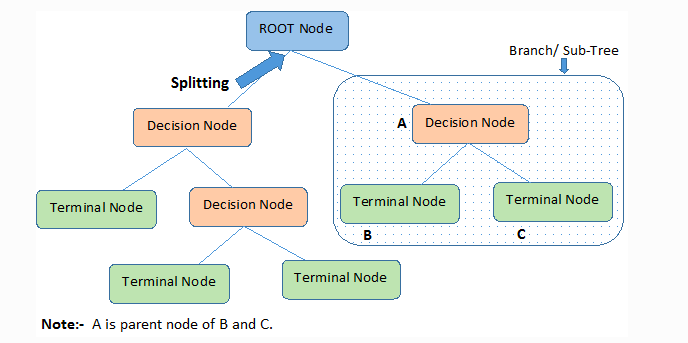
\includegraphics[width=160mm]{images/decisiontreeoverview1.png}
	\label{figdecisionalgo1} % for referencing
\end{figure}
Decision trees classify the examples by sorting them down the tree from the root to some leaf/terminal node, with the leaf/terminal node providing the classification of the example.

Each node in the tree acts as a test case for some attribute, and each edge descending from the node corresponds to the possible answers to the test case. This process is recursive in nature and is repeated for every subtree rooted at the new node.

\item \textbf{Assumptions while creating Decision Tree}\\
Below are some of the assumptions we make while using Decision tree:\\
\vspace{-18pt}
\begin{itemize}
\item In the beginning, the whole training set is considered as the root.
\item Feature values are preferred to be categorical. If the values are continuous then they are discretized prior to building the model.
\item Records are distributed recursively on the basis of attribute values.
\item Order to placing attributes as root or internal node of the tree is done by using some statistical approach.
\end{itemize}
Decision Trees follow Sum of Product (SOP) representation. The Sum of product (SOP) is also known as Disjunctive Normal Form. For a class, every branch from the root of the tree to a leaf node having the same class is conjunction (product) of values, different branches ending in that class form a disjunction (sum).

The primary challenge in the decision tree implementation is to identify which attributes do we need to consider as the root node and each level. Handling this is to know as the attributes selection. We have different attributes selection measures to identify the attribute which can be considered as the root note at each level.

\item \textbf{Reduction in Variance}\\
Reduction in variance is an algorithm used for continuous target variables (regression problems). This algorithm uses the standard formula of variance to choose the best split. The split with lower variance is selected as the criteria to split the population:\\
\textbf{Steps to calculate Varience and varience reduction:}\\
\vspace{-18pt}
\begin{enumerate}
\item Calculate variance for each node.
\item Calculate variance for each split as the weighted average of each node variance.
\item Differentiate varience of child from varience of parent. 
\end{enumerate}
\textbf{Used Formulae:}\\
Average = $\frac{\sum{x}}{n}$\\
Standard Deviation(Sd)=$\sqrt{\frac{\sum{x-\bar{x}}}{n} }$\\
Varience(var)=$\frac{1}{N}\sum{\left( {x_i - \bar x} \right)^2 } $\\
Varience Reduction= $var(parent)-\sum{w_i var(child_i)}$\\



\end{enumerate}

\subsection{Data Preprocessing}
\subsubsection{Step 1:Importing the required libraries}
These two are essential libraries which we will import every time.
Numpy is a library which contains mathematical functions.
Pandas is the library used to import and manage the data sets. 

\subsubsection{Step 2:Importing the data set}
Data sets are generally available in .csv format. A CSV file stores tabular data in plain text. Each line of the file is a data record. We use the read.csv method of the pandas library to read a local. CSV file as a data frame. Then we make separate Matrix and Vector of independent and dependent variables from the dataframe.

\subsubsection{Step 3: Handling the Missing Data}
The data we get is rarely homogeneous. Data can be missing due to various reasons and needs to be handled so that it does not reduce the performance of our machine learning model. We can replace the missing data by the Mean or Median of the entire column. We use Imputer class of sklearn.preprocessing for this task.

\subsubsection{Step 4: Encoding Categorical Data}
Categorical data are variables that contain label. values rather than numeric values. The number of possible values is often limited to a fixed set. Example values
 such as "Yes" and "No" cannot be used in mathematical equations of the model so we need to encode these variables into numbers. To achieve this we import Label Encoder class from sklearn.preprocessing library.
 
\subsubsection{Step 5: Splitting the dataset into test set and training set}
We make two partitions of dataset one for training the
model called training set and other for testing the performance of the trained model. called test set. The
split is generally $80/20$. We import train test split  method of sklearn.crossvalidation library.

\subsubsection{Step 6: Feature Scaling}
Most of the machine learning algorithms use the
71	Euclidean distance between two data points in their 
computations, features highly varying in magnitudes, units and range pose problems. High magnitudes features will weigh more in the distance calculations than features with low magnitudes. Done by Feature standardization or Z-score normalization. Standard Scalar of sklearn.preprocessing is imported.




\subsection{Steps for Decision Tree Regression Model:}
\subsubsection{Step 1:Importing the libraries}
The first step will always consist of importing the libraries that are needed to 
develop the ML model. The NumPy, matplotlib and the Pandas libraries are imported.\par
\begin{figure}[H]
	\centering
	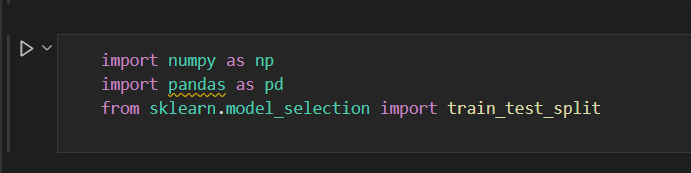
\includegraphics[width=160mm]{images/import library.png}
	\label{figimport} % for referencing
\end{figure}


\subsubsection{Step 2:Initialize and print the Dataset}
\begin{figure}[H]
	\centering
	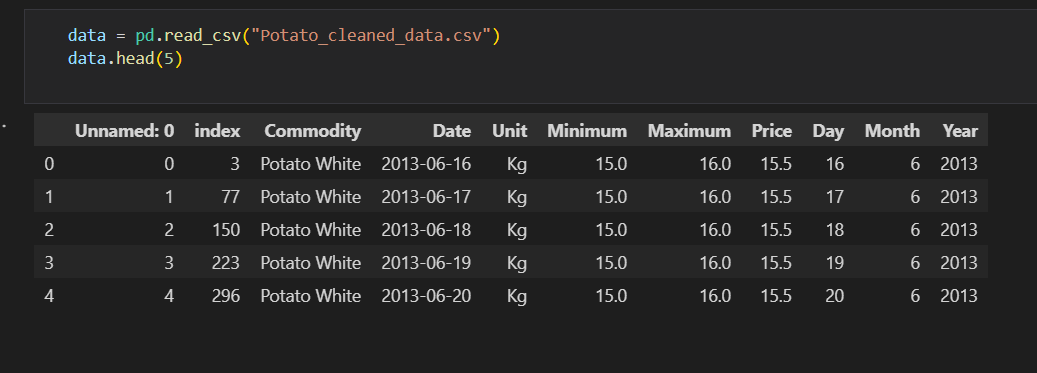
\includegraphics[width=160mm]{images/intdata.png}
	\label{figintdata} % for referencing
\end{figure}

\subsubsection{Step 3: Select all the independent features from the dataset to “X” and dependent features to "y"}
\begin{figure}[H]
	\centering
	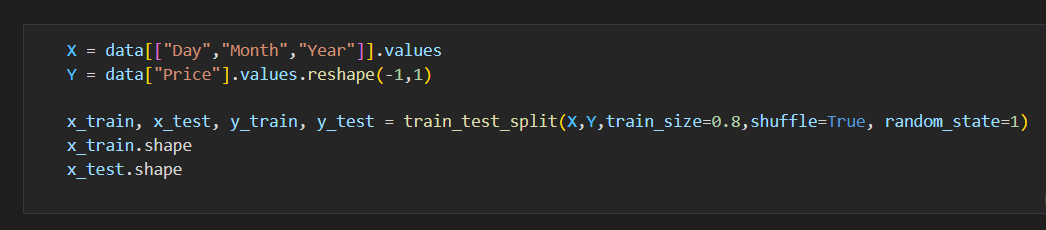
\includegraphics[width=160mm]{images/feature.png}
	\label{figfeature} % for referencing
\end{figure}

\subsubsection{Step 5: Fit decision tree regressor to the dataset}
\begin{figure}[H]
	\centering
	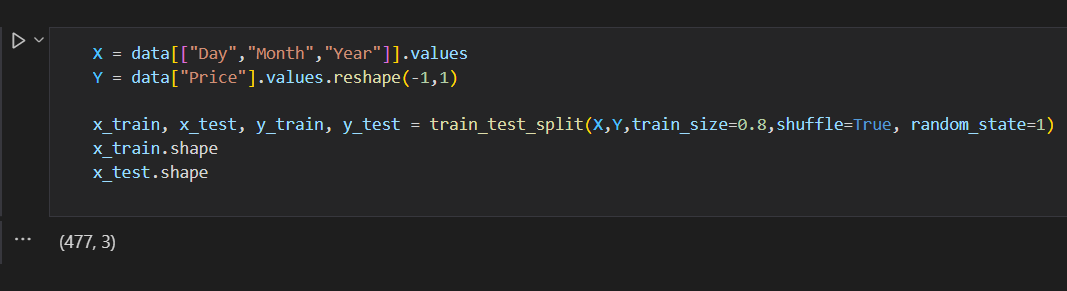
\includegraphics[width=160mm]{images/fit.png}
	\label{figfit} % for referencing
\end{figure}


\subsubsection{Step 6: Predicting a new value}
\begin{figure}[H]
	\centering
	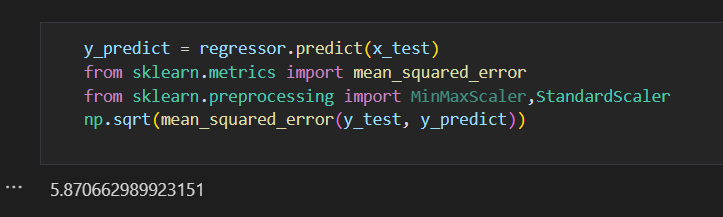
\includegraphics[width=160mm]{images/predict.png}
	\label{figpredict} % for referencing
\end{figure}


\subsubsection{Step 7: Visualising the result}
\begin{figure}[H]
	\centering
	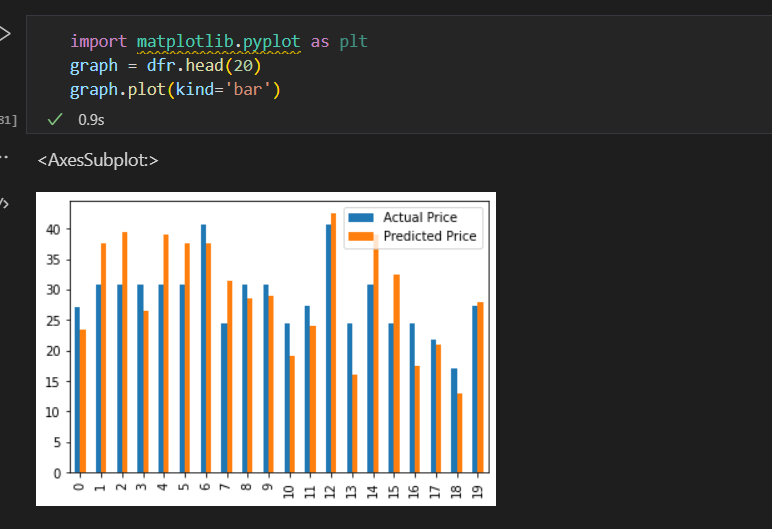
\includegraphics[width=160mm]{images/visualize.png}
	\label{figvisualize} % for referencing
\end{figure}



\section{Software development model}
\subsection{Incremental Model}
\begin{figure}[H]
	\centering
	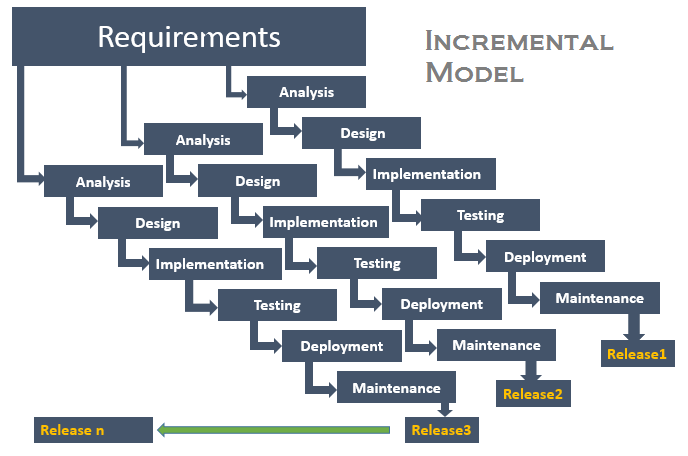
\includegraphics[width=160mm]{images/incremental model.png}{}
	\caption{Incremental Model Block Diagram} %figure name
	\label{figincremental} % for referencing
\end{figure}

\subsubsection{First Increment:}
First, the website was analyzed to know how it should look like. 
Then, the designing of templates was done. After observing the design of the 
templates, we started coding using hypertext languages Html, CSS, JavaScript, and Bootstrap. 
And finally, after testing the frontend was created.

\subsubsection{Second Increment:}
After analyzing the scenario of the project, the algorithms to be 
implemented was analyzed. Using the algorithms, we started designing 
the algorithms that is suitable for the project. Initiating the coding we 
completed the algorithm implementation. The testing of algorithm was done using the dataset. 
Finally, the algorithm was implemented.

\subsubsection{Third Increment:}
After the algorithm implementation backend designing and coding 
was started. Using Django and Python the backend part 
was completed and tested. Finally, backend was ready.

\subsubsection{Fourth Increment:}
Finally, after all the designing was completed, coding for the project was done. Later, 
testing of the project was done. 
At last, the final website was designed.

\section{Block Diagram:}
\begin{figure}[H]
	\centering
	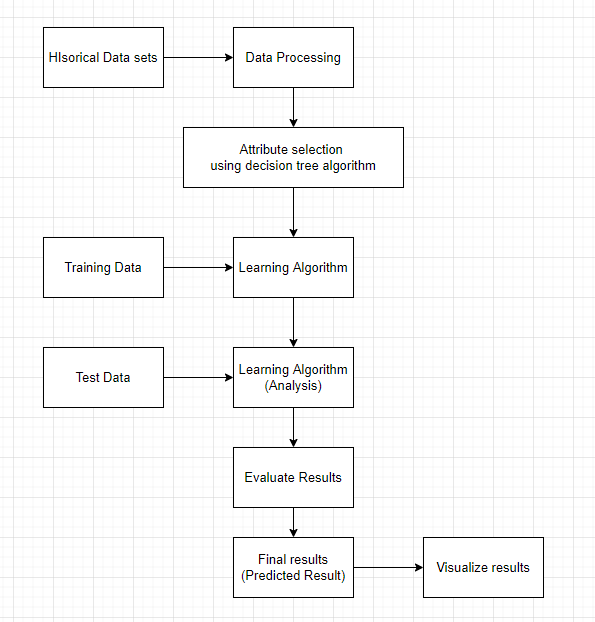
\includegraphics[width=160mm]{images/blockdiagram.png}
	\caption{Block Diagram} %figure name
	\label{figblockdiagram} % for referencing
\end{figure}

\section{Use Case Diagram:}
\begin{figure}[H]
	\centering
	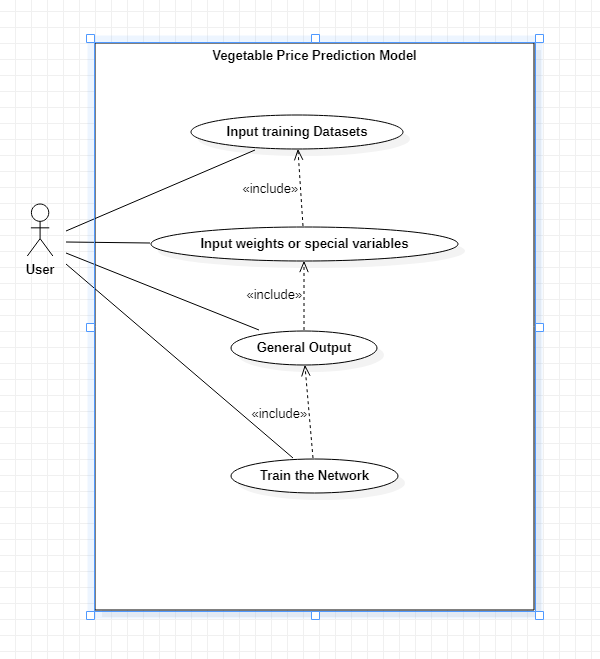
\includegraphics[width=160mm]{images/usecase.png}
	\caption{Use Case Diagram} %figure name
	\label{figusecase} % for referencing
\end{figure}




\chapter{Result and Discussion}

\section{Output:}
We succesfully created a vegetable price predictiction model which can predict price with good accuracy. All the the data to train model were taken from Kalimati market price dataset to complete our project. We use 
data from year 2013 t0 2021 and use hundreds of dats's for better accuracy of our model. 

We then trained all the datasets to make a model. We tried to create efficient and accurate model to identify the vegetable and predict it's price of the given date. After training and testing of model, a user friendly web UI is made for the user to make task easier.

Machine learning model accuracy is the measurement used to determine which model
is best at identifying relationships and patterns between variables in a data-set based on
the training data. 

In Machine Learning, error is used to see how accurately our model can predict on data it uses to learn; as well as new, unseen data.

\begin{figure}[H]
	\centering
	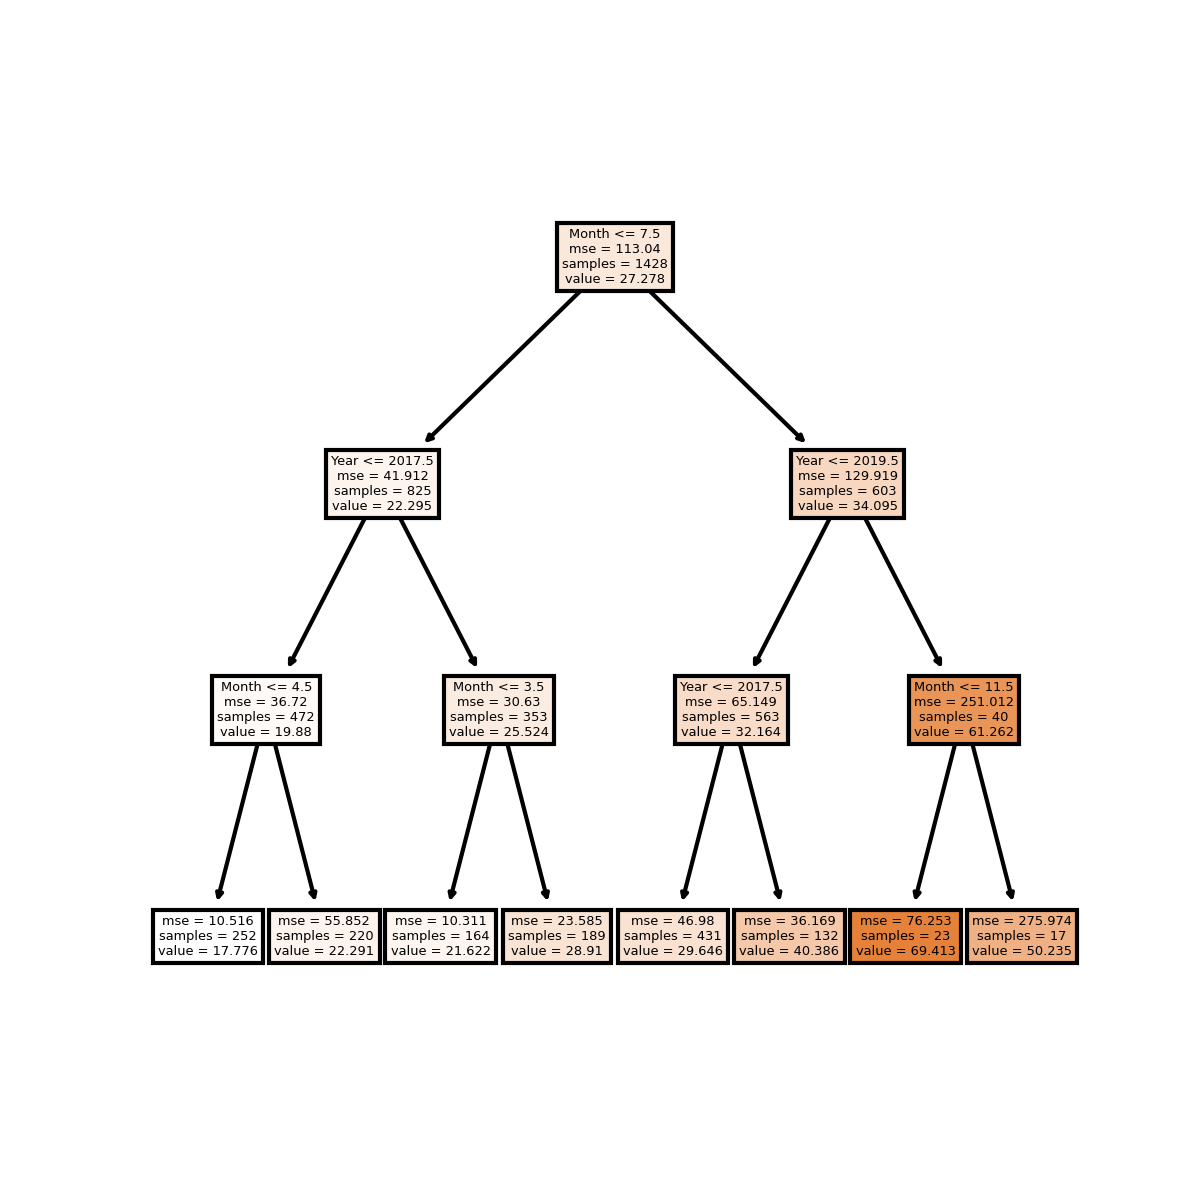
\includegraphics[width=140mm]{images/DecisionTree_1.png}
	\caption{Vegetable Price Prediction Decision Tree} %figure name
	\label{figresult} % for referencing
\end{figure}
The above figure shows the regression tree working for our model. This figure includes year, month, regreesion value etc which shows how regression tree method is working and providing us assist for creating vegetable price prediction model. 

\begin{figure}[H]
	\centering
	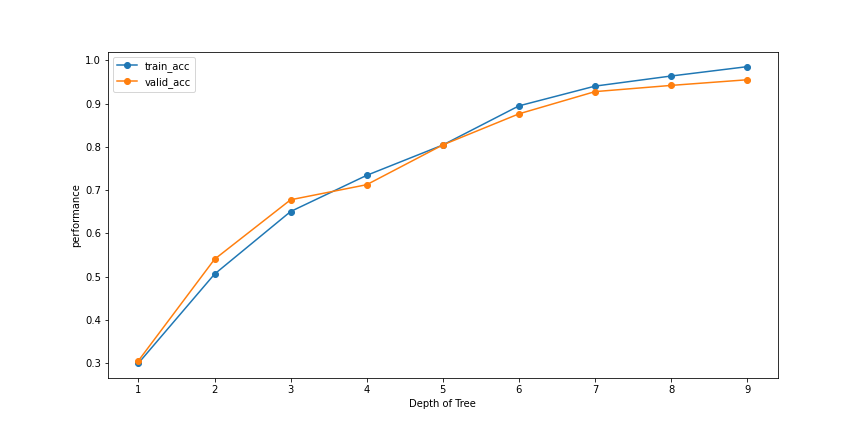
\includegraphics[width=160mm]{images/accuracy.png}
	\caption{Vegetable Price Prediction Model Accuracy} %figure name
	\label{figresult2} % for referencing
\end{figure}
The above figure shows the accuracy of our model. It has accuracy of about 75\%.

\begin{figure}[H]
	\centering
	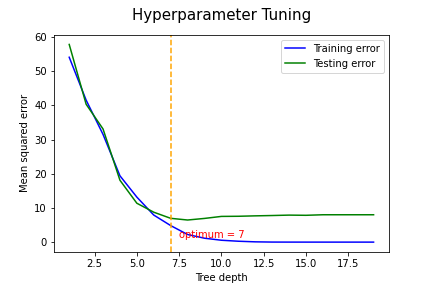
\includegraphics[width=140mm]{images/error.png}
	\caption{Vegetable Price Prediction Mode error} %figure name
	\label{result3} % for referencing
\end{figure}
The above figure shows the error of our model. We get mean square error of approximate 34.46, absolute error of approx 4.34 and mean square error of about 5.87.

\section{UI output}

\begin{figure}[H]
	\centering
	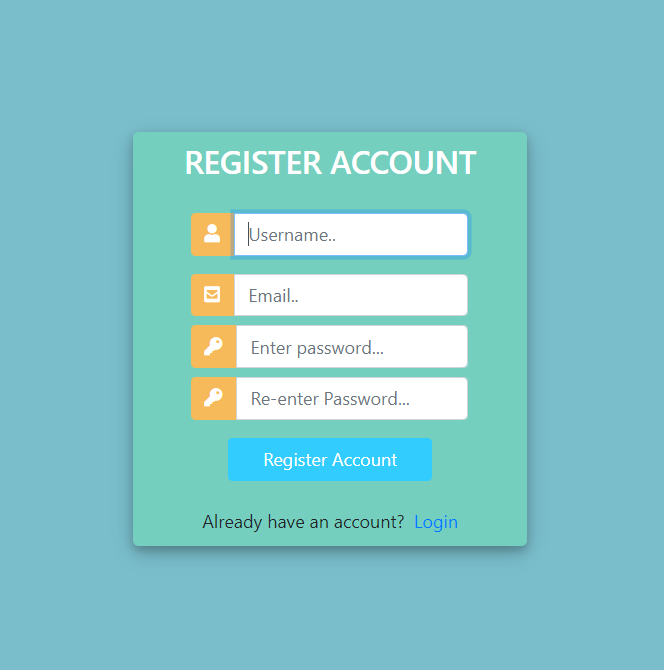
\includegraphics[scale=0.4]{images/signup.png}
	\caption{Sign up interface} %figure name
	\label{figsignup} % for referencing
\end{figure}

\begin{figure}[H]
	\centering
	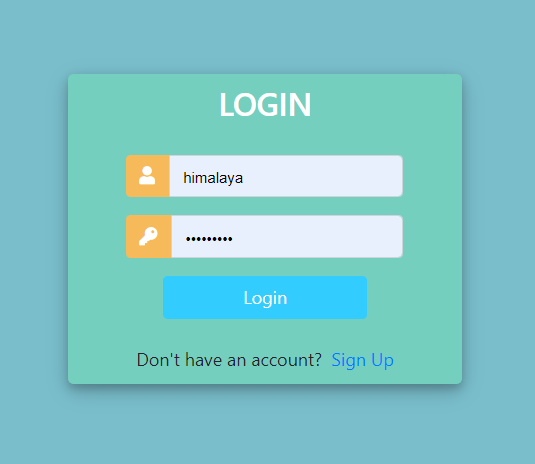
\includegraphics[scale=0.5]{images/login.png}
	\caption{Sign in interface} %figure name
	\label{figlogin} % for referencing
\end{figure}

\begin{figure}[H]
	\centering
	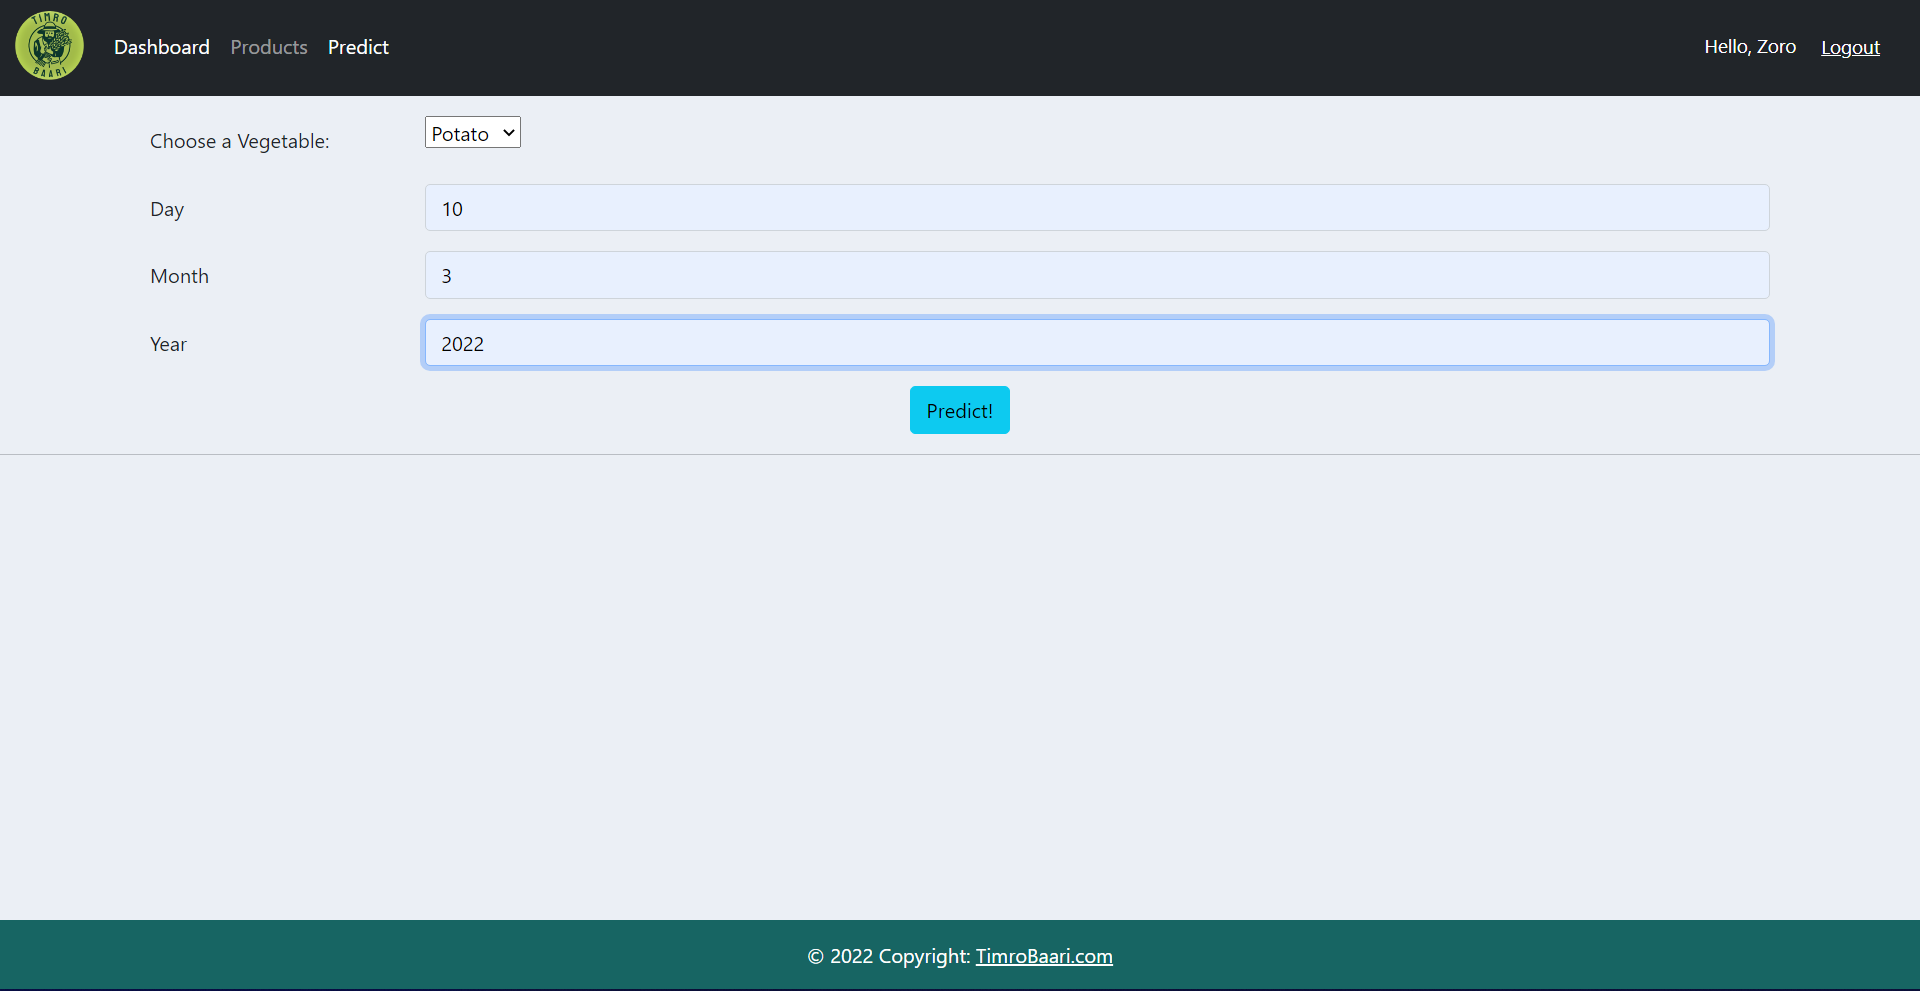
\includegraphics[width=120mm]{images/output1.png}
	\caption{Output of UI} %figure name
	\label{figoutput1} % for referencing
\end{figure}


\begin{figure}[H]
	\centering
	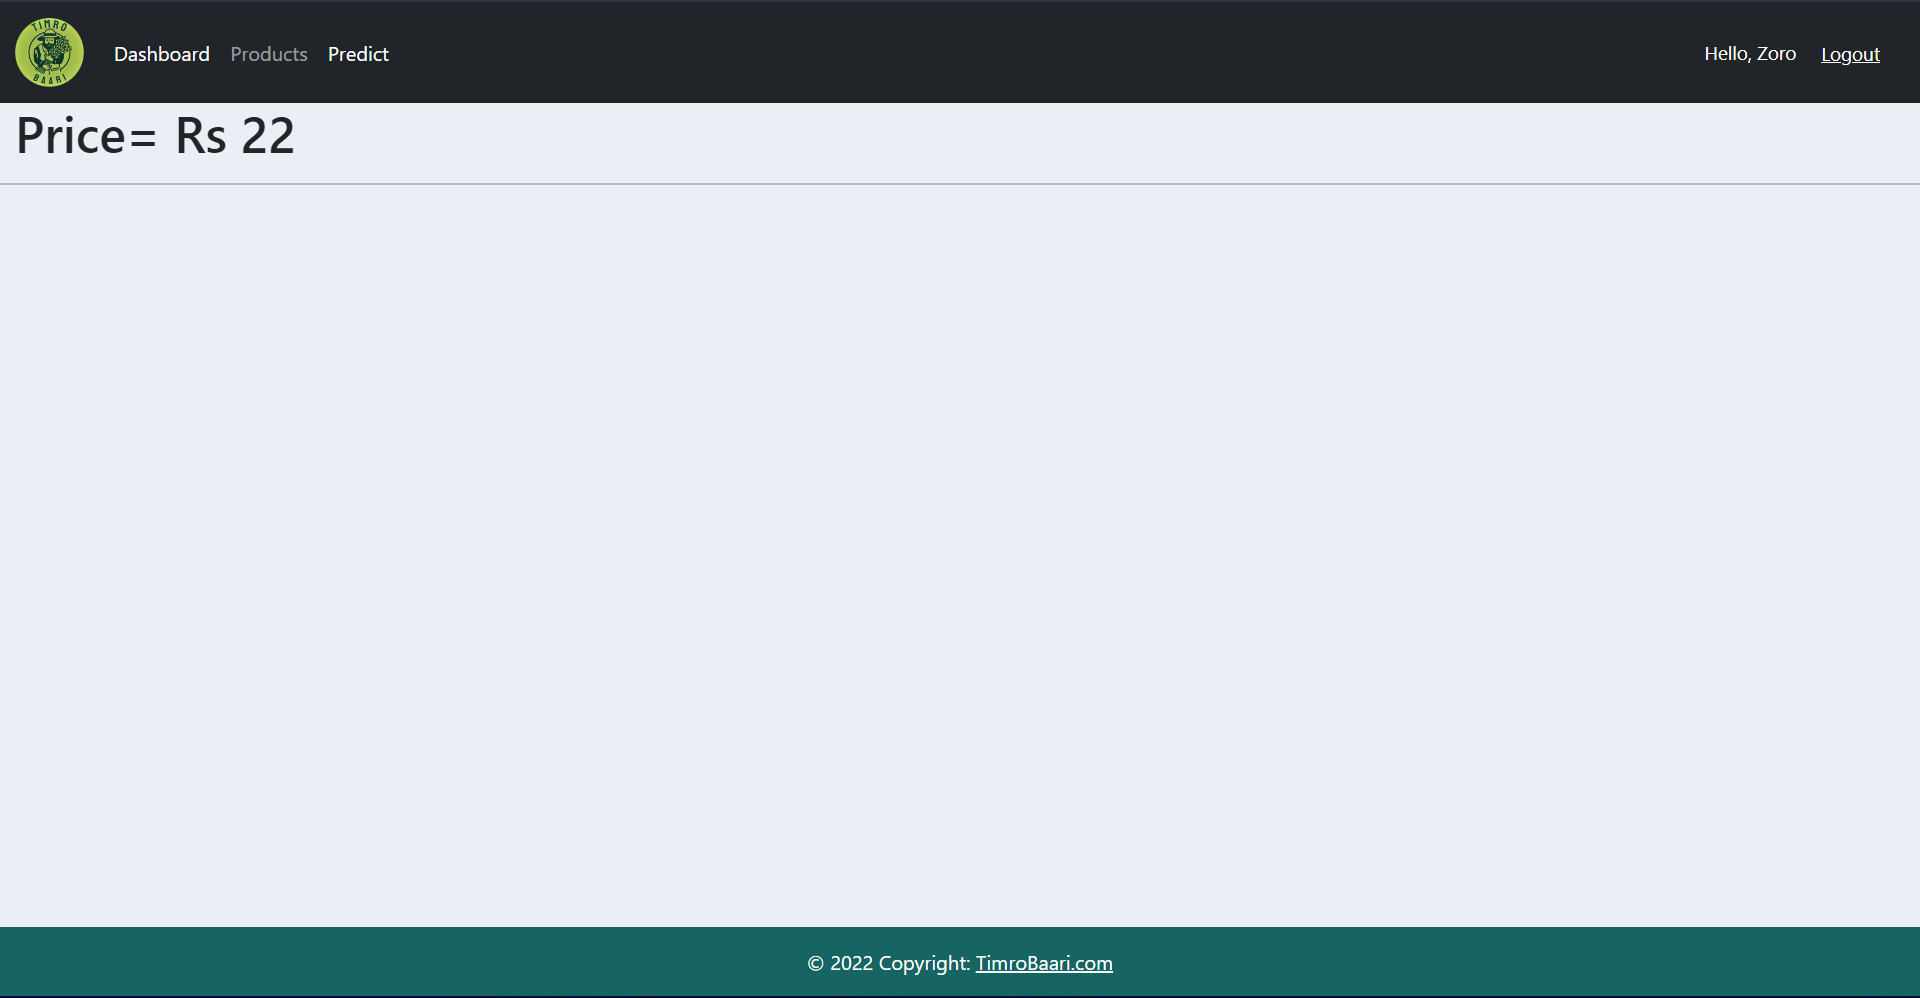
\includegraphics[width=120mm]{images/output2.png}
	\caption{Output of UI} %figure name
	\label{figoutput2} % for referencing
\end{figure}
The above figures shows the User interface of our website where we can sign up , log in and predict price of vegetables using day , month and year. 





\chapter{Conclusion}
Timro Baari (A vegetable Price Prediction Model) uses machine learning method using regression tree. It can detect the price of vegetables of given date (year/month/date) of vegtable which we choose to predict. This can help different aspects of agriculture and farmers can predict price through which they can mass produce vegetables in which they will get more profit. As well as costumer can predict price of vegetables and buy more vegetables which they need before increment of price. It will help in production of vegetables of farmers in which they will not have loss. This proposed model has accuracy of about 75%.

\subsection{Possible Future research}
In future we can use other various types of machine learning method for better accuracy of prediction. We can also add tremendous amount of datasets and more type of vegetables choice. We can also make our Web UI more user friendly and clean.   


%Reference
\renewcommand\bibname{References} % Change heading to References
\bibliographystyle{IEEEtran} % to use IEEE Format for referencing
\addcontentsline{toc}{chapter}{References} % to add references in TOC
\bibliography{library} % specify the .bib file containing reference information 

%Comment this Chapter if you do not need to include Appendix.
%\chapter*{Appendix}
%\addcontentsline{toc}{chapter}{Appendix}
%Appendix Text Comes Here

\end{document}
